\documentclass[12pt]{article}

\usepackage{sbc-template}
\usepackage{graphicx,url}
\usepackage[utf8]{inputenc}
\usepackage[brazil]{babel}
\usepackage{booktabs}
\usepackage{placeins}
\setlength{\textfloatsep}{8pt plus 2pt minus 4pt}
\setlength{\floatsep}{8pt plus 2pt minus 4pt}
\setlength{\intextsep}{8pt plus 2pt minus 4pt}
\usepackage{tikz}
\usetikzlibrary{arrows.meta}
\newcommand{\circled}[1]{\textcircled{\raisebox{-0.5pt}{\small #1}}}
\tolerance=9999
\emergencystretch=3em

\sloppy

\title{TinyML para Detecção de Doenças em Tomateiro: Três Arquiteturas de
Inferência e Gap Laboratório-Campo}

%% VERSÃO BLIND — descomentar para submissão com revisão cega
% \author{Omitido para revisão cega\inst{1}}
% \address{Instituição omitida \email{omitido@omitido.com}}

\author{[Autor Omitido para Revisão Cega]\inst{1}}

\address{[Instituição Omitida para Revisão Cega]}

\begin{document}
\maketitle

\begin{abstract}
This paper presents \textit{Ceres Diagnóstico}, a low-cost TinyML system for early
detection of tomato leaf diseases integrating distributed inference across an
embedded microcontroller, a mobile device, and a cloud API.
A MobileNetV2 INT8 model (638~KB), trained on PlantVillage (88{,}949 augmented
images) via two-phase transfer learning, is deployed across three inference
architectures:
ESP32-S3 edge (692~ms, offline), Android on-device via \texttt{tflite\_flutter}
($\approx$200--400~ms estimated, not empirically measured), and Django REST API (306~ms, cloud). Five training
experiments document the impact of INT8 calibration (+33.8~pp over the uncalibrated
model; 2.37~pp residual loss vs.\ float), synthetic background augmentation
(ineffective), and real-data fine-tuning (+10~pp). The final model achieves 98.43\%
(float) on PlantVillage and 18--30\% on three independent field datasets,
quantifying the persistent lab-field gap.

\vspace{0.5em}\noindent\textbf{Keywords:} TinyML, MobileNetV2, ESP32-S3, plant
disease detection, embedded machine learning, lab--field gap.
\end{abstract}

\begin{resumo}
Este artigo apresenta o \textit{Ceres Diagnóstico}, sistema de baixo custo para
detecção precoce de doenças foliares em tomateiro integrando TinyML, IoT e
aplicativo móvel, com inferência distribuída entre microcontrolador embarcado,
dispositivo móvel e nuvem. Um modelo MobileNetV2 INT8 (638~KB), treinado no PlantVillage
(88.949 imagens com \textit{augmentation}) via \textit{transfer learning} em duas
fases, é implantado em três arquiteturas de inferência: ESP32-S3 embarcado
(692~ms, offline), on-device no
Android via \texttt{tflite\_flutter} ($\approx$200--400~ms estimados, não medidos empiricamente) e API Django
REST (306~ms, nuvem). Cinco experimentos documentam o impacto da calibração INT8
(+33,8~pp sobre o modelo não-calibrado; 2,37~pp de perda residual vs.\ float),
\textit{augmentation} sintética (ineficaz) e \textit{fine-tuning} real (+10~pp). O modelo final atinge
98,43\% (float) no PlantVillage e 18--30\% em três \textit{datasets} de campo,
quantificando o gap laboratório-campo.

\vspace{0.5em}\noindent\textbf{Palavras-chave:} TinyML, MobileNetV2, ESP32-S3,
detecção de doenças em plantas, aprendizado de máquina embarcado, gap
laboratório-campo.
\end{resumo}


%% ----------------------------------------------------------------
\section{Introdução}
%% ----------------------------------------------------------------

O tomateiro (\textit{Solanum lycopersicum}) é uma das culturas de maior importância
econômica no Brasil, com produção anual superior a 4 milhões de toneladas
\cite{fao2024}. Doenças foliares como requeima (\textit{Phytophthora infestans}),
septoriose (\textit{Septoria lycopersici}) e mancha-bacteriana (\textit{Xanthomonas}
spp.) podem causar perdas de até 100\% da safra \cite{embrapa2023}. O diagnóstico
tradicional depende de agrônomos especializados, inacessíveis à maioria dos pequenos
produtores rurais brasileiros.

Estudos com visão computacional demonstraram acurácia elevada em condições
controladas --- Mohanty et al.~\cite{mohanty2016} atingiram 99,35\% no PlantVillage
--- mas quedas severas ao transferir modelos para o campo real: Singh et
al.~\cite{singh2020} documentaram $\approx$31\% sem adaptação de domínio e Xu et
al.~\cite{xu2024} relataram quedas de até 58~pp. Essa lacuna é aprofundada na
Seção~\ref{sec:relacionados}. Sistemas TinyML (\textit{Tiny Machine Learning})
permitem inferência de redes neurais em microcontroladores sem dependência de nuvem
\cite{warden2019} --- crítico para regiões com conectividade instável como o
Centro-Oeste brasileiro.

Este trabalho apresenta o \textbf{Ceres Diagnóstico}, que: (1)~cobre 10~classes de
doenças; (2)~demonstra, como prova de conceito, inferência no ESP32-S3 em 692~ms
com modelo de 638~KB (sem câmera integrada neste ciclo);
(3)~implementa três arquiteturas de inferência complementares (ESP32-S3, Android
on-device e API cloud) sobre o mesmo modelo; (4)~valida quantitativamente o gap em
3~\textit{datasets} independentes; (5)~documenta cinco experimentos com resultados
negativos reprodutíveis (\textit{augmentation} sintética ineficaz) e positivos
(\textit{fine-tuning} real $+$10~pp). Código e modelos disponíveis em
\url{https://anonymous.4open.science/r/extensao2-B79B}.

O desenvolvimento seguiu ciclos iterativos em contexto de projeto acadêmico de
graduação sem financiamento externo dedicado. Restrições de prazo e a não-aquisição do módulo de câmera
OV5640 no ciclo vigente impediram a conclusão do \textit{pipeline} de captura
ponta a ponta no ESP32-S3; em consequência, o caminho Mobile~(\circled{2})
tornou-se o principal veículo de validação funcional do produto neste ciclo,
enquanto o caminho Edge~(\circled{1}) permanece como prova de conceito de
inferência embarcada.

O restante deste artigo está organizado em seis seções, incluindo esta introdução.
A Seção~2 apresenta o referencial teórico (TinyML, MobileNetV2, quantização INT8 e
MQTT); a Seção~\ref{sec:relacionados} discute os trabalhos relacionados; a Seção~4
detalha a metodologia (arquitetura, treinamento, \textit{dataset} e experimentos);
a Seção~5 apresenta
e discute os resultados; e a Seção~6 traz as considerações finais e os trabalhos
futuros.


%% ----------------------------------------------------------------
\section{Referencial Teórico}
%% ----------------------------------------------------------------

\subsection{TinyML e Inferência Embarcada}

TinyML designa a execução de modelos de aprendizado de máquina em
microcontroladores com restrições severas de memória (tipicamente $<$512~KB~RAM)
e energia ($<$1~W) \cite{warden2019}. O TensorFlow Lite Micro (TFLite Micro) é o
principal \textit{framework} para esse paradigma, executando modelos quantizados
diretamente no firmware sem sistema operacional. A ausência de dependência de rede
torna o TinyML adequado para ambientes rurais com conectividade instável.
A opção por um microcontrolador (ESP32-S3, $\approx$R\$~80) em vez de um computador
de placa única (Raspberry Pi~4, $\approx$R\$~400$+$) deve-se ao menor custo, à
ausência de sistema operacional (menor superfície de ataque e \textit{boot}
instantâneo) e ao consumo reduzido ($<$500~mW vs.\ $>$5~W), viabilizando o
\textit{deploy} rural de baixo custo.

\subsection{MobileNetV2 e Quantização INT8}

O MobileNetV2 \cite{howard2017,sandler2018} introduziu os blocos
\textit{inverted residuals with linear bottleneck}, que combinam expansão de
canais, convolução depthwise separável e projeção linear. Essa arquitetura reduz
o número de parâmetros de 138M (VGG16) para 3,4M, e com fator de escala
alpha$=0{,}35$ chega a apenas 0,5M parâmetros --- compatível com a memória do
ESP32-S3.

A quantização INT8 (inteiros de 8~bits) pós-treinamento \cite{jacob2018} converte
pesos e ativações de FP32 (ponto flutuante de 32~bits) para inteiros via fatores de
escala e zero-point por tensor. Sem um
\textit{representative\_dataset} de calibração, os fatores de escala são estimados
de forma imprecisa, causando degradação severa. A Tabela~\ref{tab:modelos} compara
as principais arquiteturas de Redes Neurais Convolucionais (CNN) consideradas para
implantação no ESP32-S3.

\begin{table}[ht]
\centering
\caption{Comparativo de arquiteturas CNN para implantação no ESP32-S3.}
\label{tab:modelos}
\begin{tabular}{@{}lrrc@{}}
\toprule
\textbf{Modelo} & \textbf{Parâmetros} & \textbf{RAM} & \textbf{ESP32-S3?} \\
\midrule
VGG16           & 138M  & $>$500~MB       & Não \\
ResNet-50       & 25M   & $>$100~MB       & Não \\
EfficientNet-B0 & 5,3M  & $\approx$20~MB  & Não \\
YOLO (mínimo)   & $\approx$6M & $>$10~MB  & Não* \\
MobileNetV1     & 4,2M  & $\approx$3~MB   & Sim (inferior) \\
\textbf{MobileNetV2} & \textbf{3,4M} & \textbf{$<$4~MB} & \textbf{Sim}$^\dagger$ \\
\bottomrule
\multicolumn{4}{l}{\footnotesize *YOLO: detector de objetos (bounding box),
incompatível com classificação de folha.} \\
\multicolumn{4}{p{0.85\linewidth}}{\footnotesize $^\dagger$Para o caminho mobile
(Android), modelos como EfficientNet-Lite0 e MobileNetV3-Small também seriam
viáveis. A opção pelo mesmo MobileNetV2 INT8 foi adotada para permitir comparação
direta entre os três caminhos de inferência sobre modelo idêntico, eliminando
variáveis de arquitetura. Comparação empírica entre modelos no Android constitui
trabalho futuro.}
\end{tabular}
\end{table}

\subsection{Protocolo MQTT e IoT Agrícola}

O MQTT (\textit{Message Queuing Telemetry Transport}) \cite{oasis2019} é um
protocolo de mensageria projetado para dispositivos com recursos limitados e redes
instáveis. Opera com cabeçalho mínimo de 2~bytes e suporta três níveis de
qualidade de serviço (QoS~0, 1 e~2), tornando-o superior ao HTTP REST
(\textit{Representational State Transfer}; cabeçalho $\approx$800~bytes, sem QoS
nativo) para comunicação ESP32~→~servidor em ambientes rurais.

Estabelecidos esses fundamentos, a próxima seção posiciona o Ceres Diagnóstico
frente aos trabalhos que aplicam tais técnicas à detecção de doenças em plantas.


%% ----------------------------------------------------------------
\section{Trabalhos Relacionados}
\label{sec:relacionados}
%% ----------------------------------------------------------------

Mohanty et al.~\cite{mohanty2016} estabeleceram o estado da arte inicial com 99,35\%
de acurácia no PlantVillage, mas em condições controladas (fundo uniforme,
iluminação padronizada). Singh et al.~\cite{singh2020} introduziram o PlantDoc
(2.569~imagens de campo real, 27~espécies) e documentaram queda para
$\approx$31\% sem adaptação de domínio. Neste trabalho utiliza-se o subconjunto de
tomateiro do PlantDoc: 677~imagens (\textit{train split}) para \textit{fine-tuning}
supervisionado no Exp.~D e 676~imagens (\textit{test split}) como conjunto de
validação independente nunca visto durante treinamento (total: 1.353~imagens). A remoção manual do fundo
das imagens PlantDoc elevou a acurácia de 29,73\% para 70,53\% ($+$40,8~pp) sem
modificar o modelo~\cite{singh2020}, confirmando que redes treinadas no PlantVillage
aprendem o fundo cinza como \textit{feature} discriminativa, não as lesões.

Xu et al.~\cite{xu2024} revisaram 42~trabalhos e quantificaram o gap em 29--58~pp,
concluindo que a maioria dos modelos carece de validação em condições de campo.
Barbedo~\cite{barbedo2019} documentou especificidade geográfica severa: modelos
treinados em uma região apresentam queda significativa ao serem aplicados em
variedades e condições climáticas distintas.

O Ceres Diagnóstico se diferencia por: (a)~validação em 3~\textit{datasets} de campo
independentes em três continentes; (b)~\textit{pipeline} IoT (\textit{Internet of
Things}) com três arquiteturas de inferência (ESP32-S3, Android on-device,
API cloud) em diferentes estágios de maturidade; (c)~documentação de
5~experimentos com resultados negativos reprodutíveis \cite{pineau2021}.


%% ----------------------------------------------------------------
\section{Metodologia}
%% ----------------------------------------------------------------

Trata-se de uma pesquisa aplicada de natureza experimental, organizada em ciclos
iterativos de desenvolvimento e validação. O trabalho foi desenvolvido em uma instituição federal de ensino brasileira, sem financiamento externo dedicado. A Tabela~\ref{tab:recursos}
sumariza os recursos de \textit{hardware} e \textit{software} empregados.

\begin{table}[ht]
\centering
\caption{Recursos de hardware e software utilizados.}
\label{tab:recursos}
\begin{tabular}{@{}lll@{}}
\toprule
\textbf{Etapa} & \textbf{Recurso} & \textbf{Versão / Especificação} \\
\midrule
Treinamento  & GPU NVIDIA RTX 3060 Ti           & 8~GB VRAM, CUDA (WSL2 Ubuntu) \\
Treinamento  & Python / TensorFlow              & 3.12 / 2.x \\
\textit{Backend} & Django REST + PostgreSQL      & Python 3.13 / PostgreSQL 18 \\
Embarcado    & ESP32-S3 N16R8                   & 240~MHz, PSRAM 8~MB \\
\textit{Firmware} & PlatformIO / ESP-IDF         & 5.x \\
Aplicativo   & Flutter / \texttt{tflite\_flutter} & 0.12.1 \\
Mensageria   & MQTT (HiveMQ / Mosquitto)        & TLS, porta 8883 \\
\bottomrule
\end{tabular}
\end{table}

O custo de \textit{hardware} do nó embarcado é de aproximadamente R\$~80 (ESP32-S3).
O treinamento foi realizado utilizando uma GPU NVIDIA RTX 3060 Ti (8 GB VRAM) de uso próprio, e todo o \textit{software}
empregado é de código aberto ou gratuito, mantendo o custo total do projeto acessível
ao pequeno produtor rural.

\subsection{Arquitetura do Sistema}

O sistema implementa \textbf{três caminhos de inferência complementares} sobre o
mesmo modelo TFLite INT8 (638~KB), ilustrados na Figura~\ref{fig:arquitetura}:

\textbf{(1) Caminho Edge (ESP32-S3) — \textit{prova de conceito}:} o modelo é
executado diretamente no microcontrolador ESP32-S3~N16R8 (240~MHz, PSRAM~8~MB)
via TensorFlow Lite Micro, sem qualquer dependência de rede. O resultado é
publicado via MQTT sobre TLS ao \textit{broker} HiveMQ Cloud. A imagem e as
coordenadas GPS nunca saem do dispositivo, garantindo privacidade por design.
\textbf{Status de validação:} inferência CNN medida com 10~imagens pré-carregadas
como arrays~C (692~ms~$\pm$1~ms); o \textit{pipeline} de captura completo
(câmera~→~inferência~→~MQTT) não foi concluído neste ciclo por restrição de
prazo e pela não-aquisição do módulo OV5640.

\textbf{(2) Caminho Mobile on-device (Flutter + \texttt{tflite\_flutter}) ---
\textit{principal veículo validado}:} o mesmo modelo é carregado como
\textit{asset} no APK e executado localmente no Android via
\texttt{tflite\_flutter~0.12.1}, sem servidor. Latência estimada de 200--400~ms,
funciona \textit{offline}. O usuário alterna entre modo Local e Cloud diretamente
na tela de câmera. \textbf{Status:} \textit{pipeline} funcional câmera~→~app~→~modelo~→~resultado
validado \textit{end-to-end}; tornou-se o caminho primário de validação do produto
diante das restrições que impediram a conclusão do caminho Edge.

\textbf{(3) Caminho Cloud (Flutter + Django) --- \textit{validado end-to-end}:} o
aplicativo Flutter captura a imagem, envia via HTTPS à API Django (Railway), que
executa o mesmo modelo TFLite via Python \textit{subprocess} e retorna o
diagnóstico em JSON. \textit{Pipeline} completo câmera~→~app~→~API~→~modelo~→~resultado
validado em produção.

\begin{figure}[ht]
\centering
\begin{tikzpicture}[
  arr/.style={-{Stealth[length=2.5mm]}, thick, gray!80},
  ebox/.style={draw=blue!50,  fill=blue!7,         rounded corners=4pt,
               text width=2.8cm, minimum height=1.1cm, align=center, font=\footnotesize},
  abox/.style={draw=green!60!black, fill=green!7,  rounded corners=4pt,
               text width=2.8cm, minimum height=1.1cm, align=center, font=\footnotesize},
  cbox/.style={draw=purple!60,fill=purple!7,        rounded corners=4pt,
               text width=2.8cm, minimum height=1.1cm, align=center, font=\footnotesize},
  mbox/.style={draw=black!30, fill=black!6,         rounded corners=4pt,
               text width=9.6cm, minimum height=0.7cm, align=center,
               font=\footnotesize\bfseries},
  rebox/.style={draw=blue!50,  fill=blue!7,         rounded corners=4pt,
                text width=2.8cm, minimum height=0.8cm, align=center, font=\footnotesize},
  rabox/.style={draw=green!60!black, fill=green!7,  rounded corners=4pt,
                text width=2.8cm, minimum height=0.8cm, align=center, font=\footnotesize},
  rcbox/.style={draw=purple!60,fill=purple!7,        rounded corners=4pt,
                text width=2.8cm, minimum height=0.8cm, align=center, font=\footnotesize},
]
\node[ebox] (n1) at (0,   0) {\textbf{\circled{1} Edge}\\[3pt]
                               ESP32-S3 N16R8\\{\tiny 240\,MHz $\cdot$ PSRAM 8\,MB}};
\node[abox] (n2) at (3.8, 0) {\textbf{\circled{2} Mobile}\\[3pt]
                               Android\\{\tiny tflite\_flutter 0.12.1}};
\node[cbox] (n3) at (7.6, 0) {\textbf{\circled{3} Cloud}\\[3pt]
                               Flutter + Django\\{\tiny Railway $\cdot$ HTTPS}};
\node[mbox] (model) at (3.8,-2.2)
  {MobileNetV2 INT8 $\cdot$ 638\,KB $\cdot$ $96{\times}96{\times}3$
   $\cdot$ 10 classes $\cdot$ $T{=}0{,}25$};
\node[rebox] (r1) at (0,   -3.9) {692\,ms $\pm$1\,ms\\{\tiny offline $\cdot$ MQTT/TLS}};
\node[rabox] (r2) at (3.8, -3.9) {$\approx$200--400\,ms\\{\tiny offline $\cdot$ toggle UI}};
\node[rcbox] (r3) at (7.6, -3.9) {306\,ms\\{\tiny cloud $\cdot$ PostgreSQL}};
\draw[arr, blue!70]        (n1.south) -- ++(0,-0.35)
    -| ([xshift=-3.8cm]model.north);
\draw[arr, green!60!black] (n2.south) -- (model.north);
\draw[arr, purple!70]      (n3.south) -- ++(0,-0.35)
    -| ([xshift=3.8cm]model.north);
\draw[arr] ([xshift=-3.8cm]model.south) |- (r1.north);
\draw[arr] (model.south) -- (r2.north);
\draw[arr] ([xshift= 3.8cm]model.south) |- (r3.north);
\end{tikzpicture}
\caption{Três caminhos de inferência sobre o mesmo modelo MobileNetV2 INT8 (638\,KB).
         \textbf{\circled{1}~Edge:} TFLite Micro no ESP32-S3, imagens como arrays~C
         (latência CNN pura, sem sensor).
         \textbf{\circled{2}~Mobile:} \texttt{tflite\_flutter} on-device, offline total.
         \textbf{\circled{3}~Cloud:} API Django (Railway), Python subprocess TFLite.}
\label{fig:arquitetura}
\end{figure}

\subsection{Treinamento do Modelo}

\textbf{Configuração:} MobileNetV2 alpha$=0{,}35$, entrada 96$\times$96$\times$3~RGB,
backbone pré-treinado ImageNet, cabeça: GlobalAveragePooling + Dropout(0,3) +
Dense(10, softmax).

\textbf{Treinamento em duas fases:} Fase~1 (10~épocas, LR$=1\!\times\!10^{-3}$) ---
backbone congelado, cabeça treinada; acurácia de validação estabiliza em 87,4\%.
Fase~2 (40~épocas, LR$=5\!\times\!10^{-4}$) --- últimas 30~camadas descongeladas,
EarlyStopping($p=8$) + ReduceLROnPlateau($f=0{,}5$). A melhor acurácia de validação
(97,90\%) ocorre na época~46, como ilustra a Figura~\ref{fig:treino}.

\begin{figure}[ht]
\centering
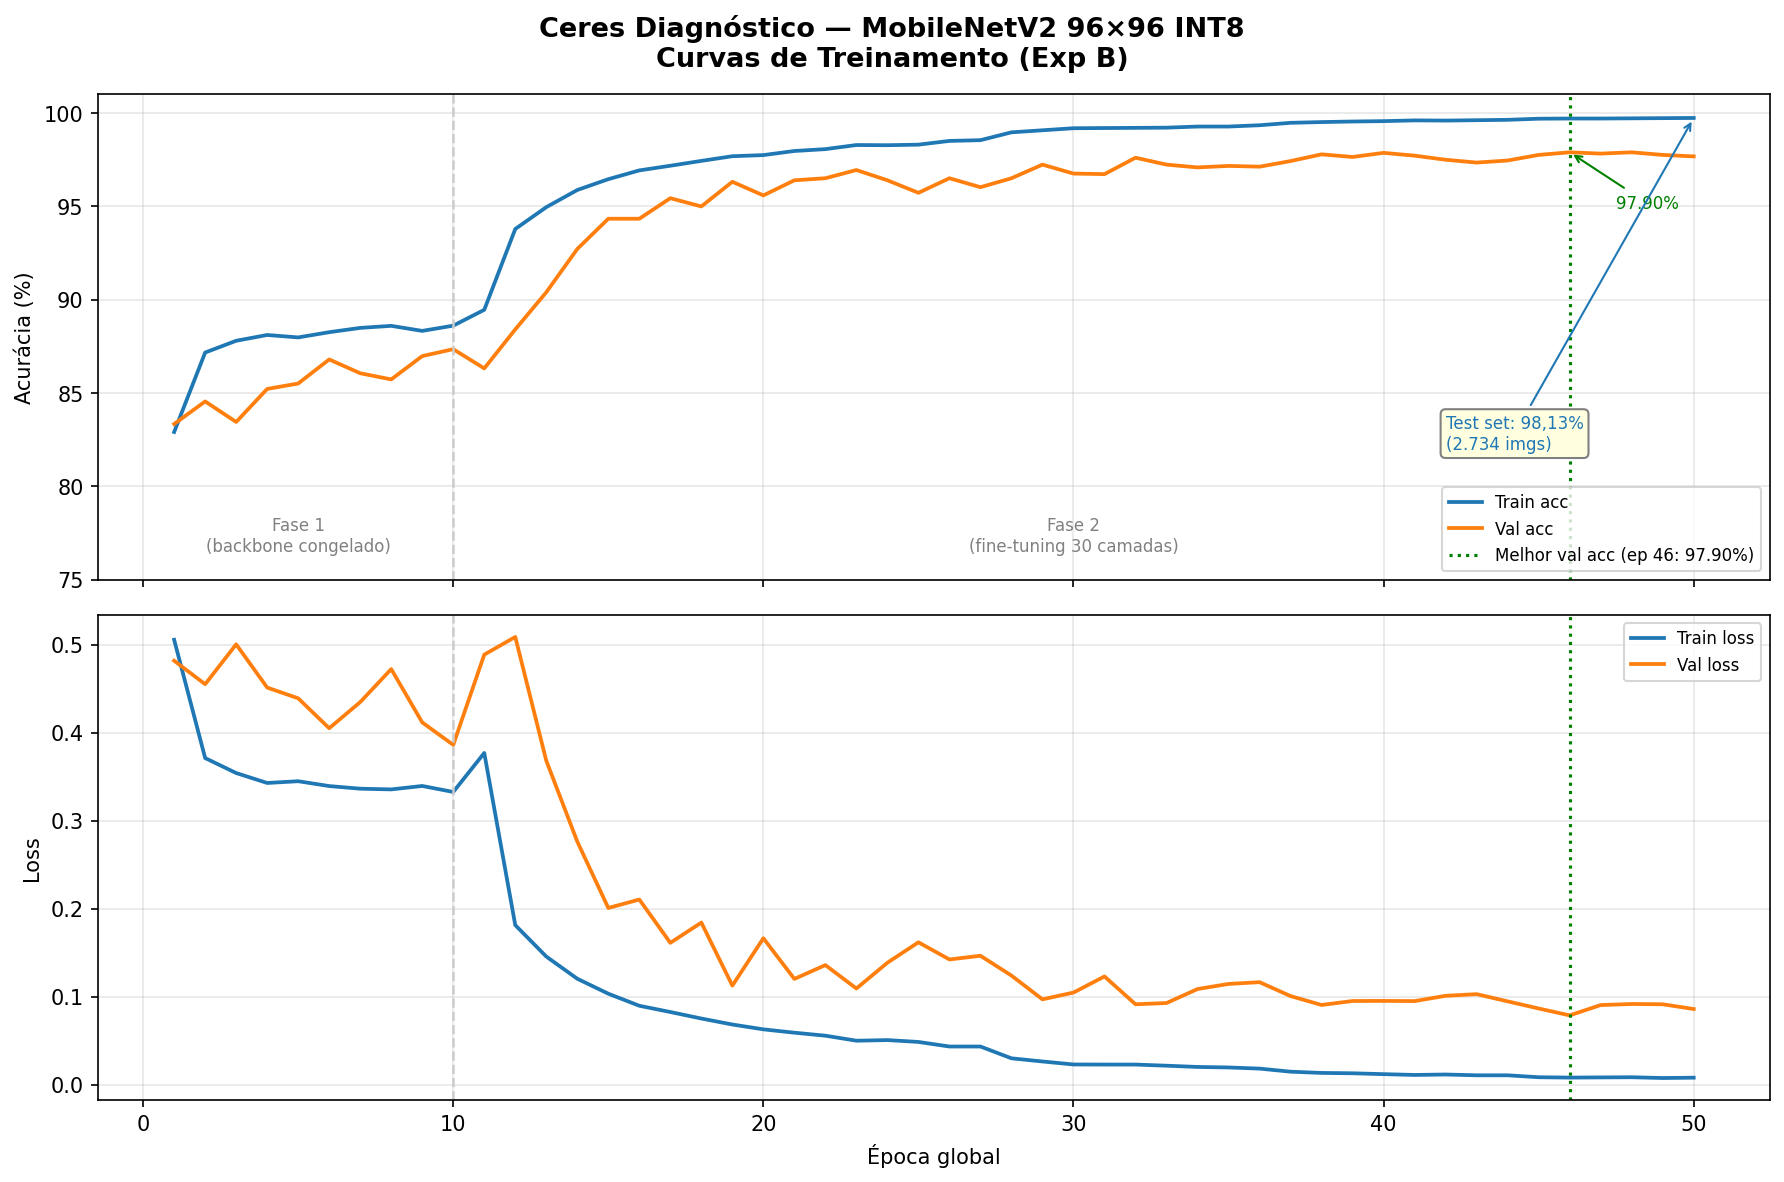
\includegraphics[width=0.92\textwidth]{historico_treino.png}
\caption{Curvas de treinamento do Exp.~B (MobileNetV2 96$\times$96). A linha vertical
tracejada marca a transição da Fase~1 (\textit{backbone} congelado) para a Fase~2
(\textit{fine-tuning} das últimas 30~camadas). A melhor acurácia de validação
(97,90\%, época~46) corresponde a 98,13\% no \textit{test set} para o modelo float.}
\label{fig:treino}
\end{figure}

\textbf{Quantização INT8 calibrada:} 50~batches do \textit{val set} como
\textit{representative\_dataset} \cite{jacob2018}. Sem calibração, a quantização
degrada a acurácia em $-$30,5~pp (Exp.~A); com calibração, a perda residual cai
para apenas 2,37~pp (98,13\% float $\to$ 95,76\% INT8 no \textit{test set}).
\textbf{Pós-processamento:} \textit{temperature scaling} \cite{guo2017} divide os
logits por um fator $T$ antes do softmax, calibrando a confiança das predições sem
alterar a classe predita. O valor $T{=}0{,}25$ foi determinado empiricamente no
\textit{val set} para maximizar a separação entre a classe correta e as demais;
aplicado de forma idêntica nos três caminhos de inferência.

\subsection{Dataset}

\textbf{PlantVillage} \cite{hughes2015}: 18.160~imagens, 10~classes, CC~BY~4.0.
\textit{Split} estratificado (seed$=42$): 70\% treino / 15\% val / 15\% teste.
\textit{Augmentation} \textit{offline} (só treino): \textit{flip} H/V, rotação $\pm$15°, brilho $\pm$20\%.
Resultado: 88.949~imagens de treino.

\textbf{Datasets de campo real} (validação independente):
PlantDoc \cite{singh2020} --- 1.353~imagens (EUA/Europa);
Tomato-Village \cite{gehlot2023} --- 217~imagens (Rajastão, Índia);
Daffodil~BD~\cite{daffodilbd2024} --- 1.616~imagens (Bangladesh).

\subsection{Experimentos}

Cinco experimentos documentam a evolução do modelo (Tabela~\ref{tab:experimentos}).

\begin{table}[ht]
\centering
\caption{Configuração dos cinco experimentos de treinamento.}
\label{tab:experimentos}
\begin{tabular}{@{}llp{5.5cm}@{}}
\toprule
\textbf{Exp.} & \textbf{Plataforma} & \textbf{Estratégia principal} \\
\midrule
A & Edge Impulse (nuvem) & Sem calibração INT8 \\
B & TF local WSL2 & 2 fases + calibração INT8 (50 batches) \\
C & TF local WSL2 & Exp.~B + background aug.\ sintética (rembg U2-Net) \\
D & TF local WSL2 & Exp.~B + fine-tuning com PlantDoc/train real \\
E & TF local WSL2 & Exp.~D + Focal Loss ($\gamma=2$) + aug.\ agressiva \\
\bottomrule
\end{tabular}
\end{table}

\subsection{Firmware, Pipeline IoT e Integração Mobile}

Firmware PlatformIO/ESP-IDF~5.x: modelo carregado como array~C no flash, arena de
inferência em PSRAM (200~KB de 512~KB alocados). A opção por imagens pré-carregadas
como arrays~C --- em vez da câmera OV5640 --- foi adotada por duas razões
complementares: isolar a latência da CNN pura da latência de captura do sensor,
garantindo medição comparável à literatura; e o fato de que a integração física
da câmera OV5640 não foi concluída dentro do prazo disponível para este ciclo de
desenvolvimento. A câmera constitui etapa futura de integração (item~iii dos
trabalhos futuros). O resultado da inferência CNN é publicado via
MQTT com QoS~1 (\textit{Quality of Service}) ao \textit{broker} HiveMQ Cloud
(porta~8883, TLS); Mosquitto local utilizado apenas em desenvolvimento. O aplicativo
Flutter captura a coordenada GPS (\textit{Global Positioning System}) antes de cada
inferência. O \textit{cache} local é gerenciado pelo Drift (SQLite) com
\texttt{SyncService}, que reenvia diagnósticos pendentes ao restaurar conectividade
(\textit{offline-first}).

A próxima seção apresenta os resultados obtidos com os cinco experimentos, a latência
medida no ESP32-S3, o comparativo entre os três caminhos de inferência e a análise
do gap laboratório-campo nos três \textit{datasets} de campo.


%% ----------------------------------------------------------------
\section{Resultados e Discussão}
%% ----------------------------------------------------------------

\subsection{Impacto da Calibração INT8}

\begin{table}[ht]
\centering
\caption{Comparativo Exp.~A (Edge Impulse) vs.\ Exp.~B (TensorFlow local).
O modelo efetivamente embarcado no ESP32-S3 é o INT8.}
\label{tab:ab}
\begin{tabular}{@{}lrrrr@{}}
\toprule
\textbf{Métrica} & \textbf{Exp.~A FP32} & \textbf{Exp.~A INT8} & \textbf{Exp.~B float} & \textbf{Exp.~B INT8} \\
\midrule
Acurácia val set  & 92,5\% & 62,0\% & 97,90\% & --- \\
Acurácia test set & ---    & ---    & 98,13\% & \textbf{95,76\%} \\
Macro F1          & 0,92   & 0,62   & 0,977   & --- \\
Tamanho modelo    & 1.637~KB & 547~KB & ---    & \textbf{638~KB} \\
\bottomrule
\end{tabular}
\end{table}

A ausência de \textit{representative\_dataset} no Exp.~A causou queda de 30,5~pp
(92,5\%~$\to$~62,0\%), consistente com Jacob et al.~\cite{jacob2018}.
Ressalta-se que Exp.~A e Exp.~B diferem não apenas na calibração INT8, mas também
em plataforma (Edge Impulse vs.\ TensorFlow local), estratégia de treinamento
(uma fase vs.\ duas fases) e hiperparâmetros; o efeito isolado da calibração não
pode ser separado dessas demais variáveis. As classes mais
afetadas foram D01\_requeima ($-$30,7~pp) e D03b\_mancha\_alvo ($-$28,6~pp) ---
as com menos amostras no \textit{val set}, evidenciando que a representatividade do
\textit{dataset} de calibração determina diretamente a qualidade dos fatores de
escala por tensor.

O Exp.~B, com calibração sobre 50~batches reais, reduz a perda de quantização a
apenas 2,37~pp: o modelo float atinge 98,13\% e o INT8 embarcado, 95,76\% no
\textit{test set} --- ainda assim $+$33,8~pp acima do INT8 não-calibrado do Exp.~A
(62,0\%). A Figura~\ref{fig:matriz} detalha os acertos e as confusões por classe do
modelo INT8.

\begin{figure}[ht]
\centering
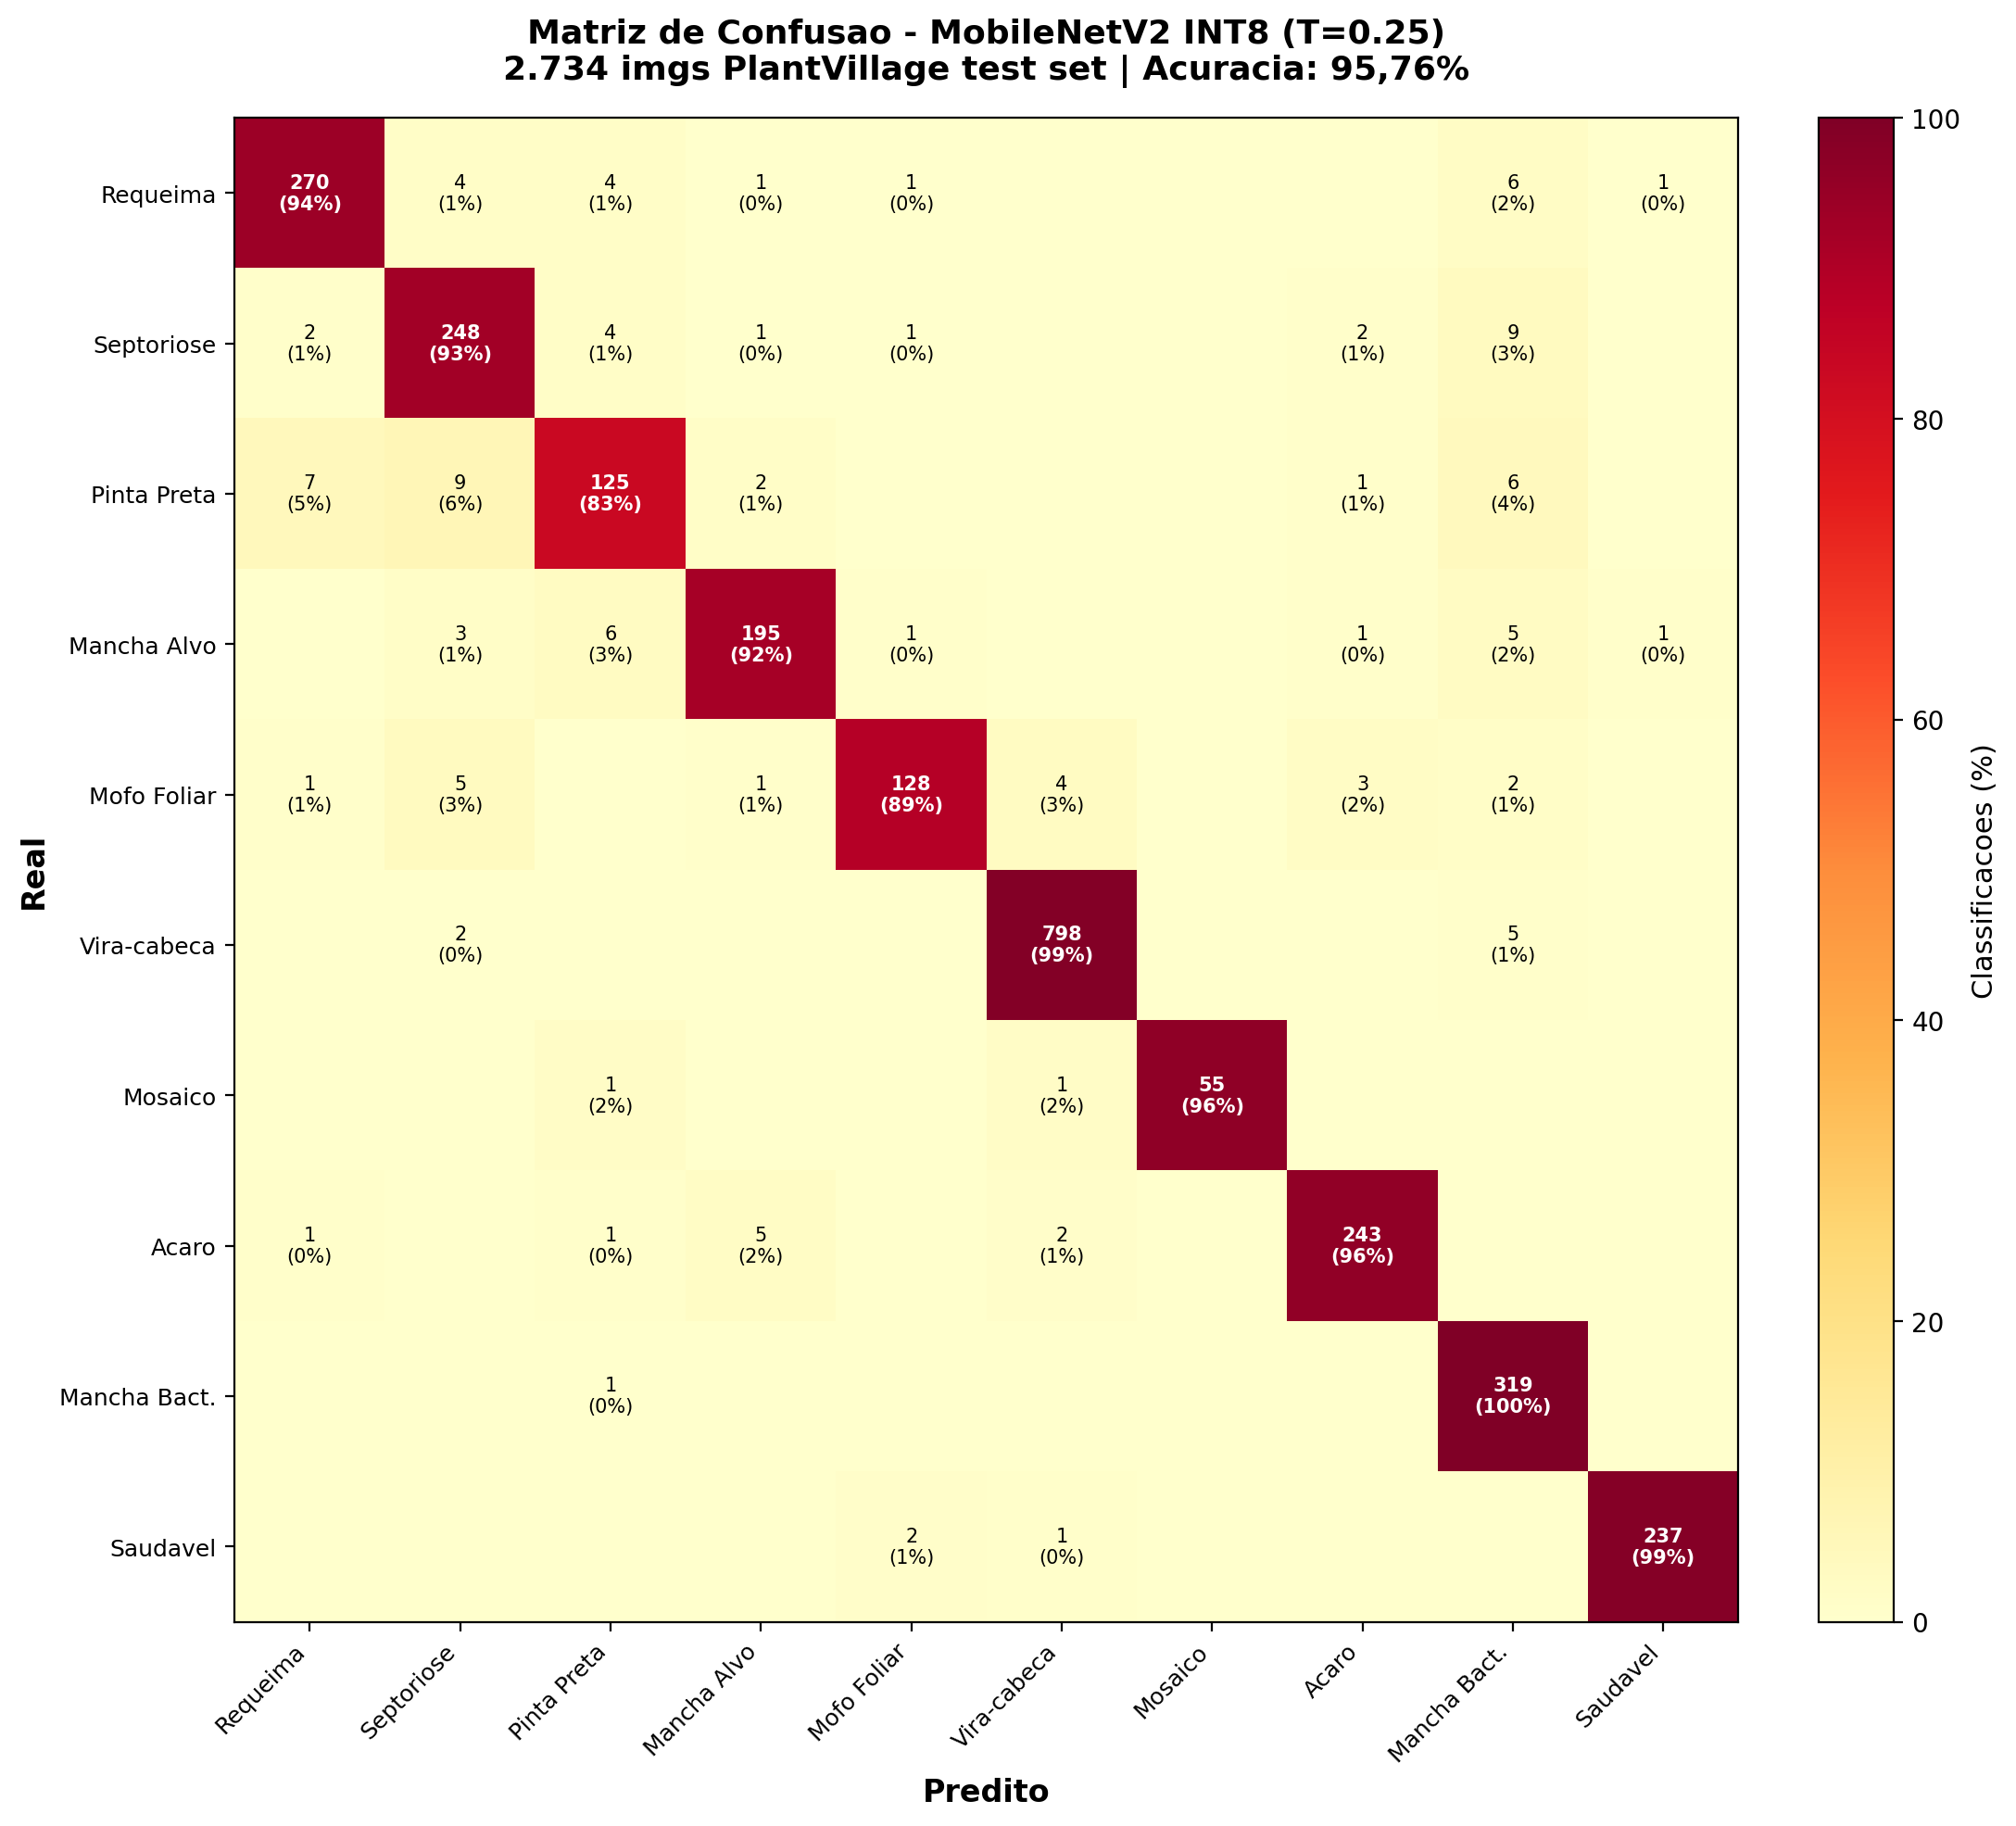
\includegraphics[width=0.78\textwidth]{matriz_confusao_int8.png}
\caption{Matriz de confusão do modelo INT8 ($T=0{,}25$) no \textit{test set} do
PlantVillage (2.734~imagens, acurácia 95,76\%). As maiores confusões ocorrem entre
pinta-preta, septoriose e requeima --- doenças com lesões necróticas visualmente
semelhantes.}
\label{fig:matriz}
\end{figure}

\FloatBarrier
\subsection{Latência no ESP32-S3}

A latência medida foi de \textbf{692~ms} ($\pm$1~ms, determinístico), com
10/10~imagens corretas (imagens pré-carregadas como arrays~C, sem câmera).
O fator limitante é a ausência de unidade SIMD
(\textit{Single Instruction, Multiple Data}) INT8 dedicada no Xtensa~LX7 ---
convoluções executadas via instruções escalares de propósito geral. No contexto
agrícola, 692~ms representa apenas a etapa de inferência CNN; o tempo total de
uso incluiria captura e posicionamento da folha, etapa não medida neste ciclo
--- tornando a latência da CNN provavelmente não o gargalo principal quando o
\textit{pipeline} de captura for concluído e validado empiricamente.

\subsection{Gap Laboratório-Campo}

\begin{table}[ht]
\centering
\caption{Acurácia por experimento em lab e campo (três datasets independentes).}
\label{tab:gap}
\begin{tabular}{@{}lcccc@{}}
\toprule
\textbf{Exp.} & \textbf{PlantVillage} & \textbf{PlantDoc} & \textbf{Tomato-Village} & \textbf{Daffodil~BD} \\
              & \textbf{(lab)}        & \textbf{(campo)}  & \textbf{(campo)}        & \textbf{(campo)} \\
\midrule
B -- baseline        & 98,13\% & 20,77\% & ---              & --- \\
C -- aug.\ sintét.   & 96,20\% & 20,24\% & ---              & --- \\
D -- fine-tun.\ real & 97,55\% & \textbf{30,43\%} & 11,52\% & --- \\
E -- Focal Loss      & \textbf{98,43\%} & 30,43\% & \textbf{27,65\%} & \textbf{18,13\%} \\
\bottomrule
\multicolumn{5}{p{0.95\linewidth}}{\footnotesize Coluna lab: acurácia do modelo
float no \textit{test set}; o INT8 embarcado do Exp.~B atinge 95,76\%
(Fig.~\ref{fig:matriz}). Colunas de campo: modelo INT8 (mesma quantização do ESP32-S3).}
\end{tabular}
\end{table}

Tomato-Village e Daffodil~BD foram avaliados apenas nos modelos finais (Exp.~D e~E),
como teste adicional de generalização geográfica; os experimentos B e~C, anteriores,
não foram reexecutados sobre eles --- daí as células~``---'' na Tabela~\ref{tab:gap}.

\textbf{Background augmentation sintética (Exp.~C):} remoção de fundo com
U2-Net~\cite{qin2020} e recomposição sobre fundos do PlantDoc não melhorou o
desempenho de campo ($+$0~pp vs.\ Exp.~B). Mesmo após 177.698~composições
sintéticas, o modelo nunca prediz folha saudável em campo (0,0\%), indicando que
o domínio sintético não captura a distribuição real. Resultado negativo
documentado segundo as diretrizes de Pineau et al.~\cite{pineau2021}.

\textbf{Fine-tuning com dados reais (Exp.~D):} 677~imagens do PlantDoc/train
(\textit{oversampling} 10$\times$, sem dados adicionais) produziram ganho de
$+$10~pp (20,77\%~$\to$~30,43\%) avaliado no PlantDoc/test (676~imagens
nunca usadas em treinamento). O fator limitante é o \textbf{volume de dados de
campo}, não o método.

\textbf{Focal Loss (Exp.~E):} Focal Loss ($\gamma=2$)~\cite{lin2017} melhorou
consistência entre \textit{datasets} ($+$16~pp no Tomato-Village: 11,52\%~$\to$~27,65\%).

\textbf{Gap geográfico:} EUA/Europa (30,43\%) $>$ Índia (27,65\%) $>$ Bangladesh
(18,13\%), confirmando Barbedo~\cite{barbedo2019}: especificidade geográfica em
função de variedades locais e condições tropicais.

\textbf{Colapso de classe:} na análise da distribuição de predições do Exp.~D
sobre o Tomato-Village, 73\% das folhas da classe saudável foram erroneamente
classificadas como D02\_septoriose --- padrão típico de colapso sob \textit{shift}
de domínio extremo, parcialmente mitigado no Exp.~E com Focal Loss ($\gamma=2$),
que penaliza predições excessivamente confiantes em classes dominantes.

\subsection{Comparativo Edge, Mobile e Cloud}

\begin{table}[ht]
\centering
\caption{Comparativo dos três caminhos de inferência.}
\label{tab:edge}
\begin{tabular}{@{}lccc@{}}
\toprule
\textbf{Aspecto} & \textbf{Edge -- ESP32-S3} & \textbf{Mobile -- Android} & \textbf{Cloud -- Django} \\
\midrule
Latência inferência & 692~ms ($\pm$1~ms)   & $\approx$200--400~ms$^*$ & 306~ms (subprocess) \\
Latência end-to-end & 692~ms               & $\approx$200--400~ms$^*$ & 2.333~ms (HTTP dev) \\
Funciona offline    & \textbf{Sim}         & \textbf{Sim}             & Não \\
Privacidade (LGPD)  & \textbf{Total}       & \textbf{Total}           & Imagem transmitida \\
Custo adicional     & $\approx$R\$~80      & Zero (app)               & Servidor PC/cloud \\
\midrule
Status validação    & Parcial$^{**}$       & \textbf{End-to-end}      & \textbf{End-to-end} \\
\bottomrule
\multicolumn{4}{p{0.9\linewidth}}{\footnotesize $^*$Estimada com base em
benchmarks públicos de \texttt{tflite\_flutter}~0.12.1 em dispositivos
\textit{mid-range}; não medida empiricamente neste ciclo por restrição de tempo
--- constitui trabalho futuro (item~iv).} \\
\multicolumn{4}{p{0.9\linewidth}}{\footnotesize $^{**}$Inferência CNN validada
(692~ms, 10~imagens); \textit{pipeline} câmera~→~inferência~→~MQTT não concluído
por restrição de prazo e não-aquisição do módulo OV5640 neste ciclo.}
\end{tabular}
\end{table}

Quando o pipeline de captura do ESP32-S3 for concluído (câmera OV5640
integrada), o caminho Edge será superior para zonas rurais sem conectividade e
cenários de privacidade total. No ciclo atual, o caminho Mobile é o único com
validação end-to-end funcional offline. A latência Cloud de 2.333~ms reflete
servidor de desenvolvimento (\textit{single-thread}); estima-se $<$200~ms em
produção com Gunicorn \textit{multi-worker}.


%% ----------------------------------------------------------------
\section{Considerações Finais}
%% ----------------------------------------------------------------

O Ceres Diagnóstico demonstrou a viabilidade técnica de uma arquitetura TinyML
distribuída --- MobileNetV2 INT8 (638~KB) validado no ESP32-S3 (692~ms,
prova de conceito) e em produção via mobile e cloud (end-to-end). Contudo, a acurácia de campo de
18--30\% em três \textit{datasets} independentes evidencia que o sistema não está
pronto para implantação produtiva: dados de campo representativos e
\textit{domain adaptation} constituem pré-requisitos para uso agrícola real.
As principais contribuições são:

\begin{enumerate}
  \item \textbf{Pipeline reproduzível:} PlantVillage $\to$ 88.949~imgs $\to$
        MobileNetV2 INT8 $\to$ ESP32-S3, código aberto
        (\url{https://anonymous.4open.science/r/extensao2-B79B}).
  \item \textbf{Quantificação da calibração INT8:} $+$34~pp com
        \textit{representative\_dataset} (62,0\%~$\to$~95,76\%) vs.\ quantização
        automática, com perda residual de apenas 2,37~pp frente ao modelo float.
  \item \textbf{Benchmark em 3 \textit{datasets} de campo:} documentação do gap
        lab-campo (98,43\%~$\to$~18--30\%) e sua natureza geográfica.
  \item \textbf{Resultado negativo reprodutível:} \textit{augmentation} sintética
        ineficaz; \textit{fine-tuning} com dados reais confirma volume como fator
        limitante.
  \item \textbf{Três arquiteturas de inferência comparadas:} ESP32-S3, Android
        on-device e API cloud sobre o mesmo modelo INT8.
\end{enumerate}

\textbf{Limitações:} A latência de 692~ms ficou acima da meta de 300~ms
(Xtensa~LX7 sem acelerador SIMD INT8). A câmera OV5640 não foi integrada neste
ciclo --- a validação usou imagens embarcadas como arrays~C. O gap
laboratório-campo (98,43\%~$\to$~18--30\%) persiste como problema aberto.

O projeto foi concebido originalmente com o ESP32-S3 como produto primário.
Ao longo do desenvolvimento, duas restrições impediram a conclusão do
\textit{pipeline} embarcado ponta a ponta: (a)~\textbf{prazo} --- o semestre
letivo não comportou a integração completa do firmware de captura;
(b)~\textbf{recurso de hardware} --- o módulo de câmera OV5640 não foi adquirido
e integrado no período disponível. Como resultado, o caminho Edge permaneceu como
prova de conceito (inferência CNN validada, latência medida), e o caminho Mobile
(Android + \texttt{tflite\_flutter}) passou a ser o principal veículo de
validação funcional do produto. Essa reorientação de escopo é documentada de
forma transparente para que os resultados sejam interpretados corretamente: as
contribuições de \textit{pipeline} reproduzível, calibração INT8 e gap
laboratório-campo são válidas e independentes do caminho de inferência; a
validação de produto completo com câmera embarcada constitui etapa futura.
Adicionalmente, a comparação entre modelos no caminho mobile limitou-se ao
MobileNetV2 por restrição de tempo; alternativas como MobileNetV3-Small e
EfficientNet-Lite0 não foram avaliadas.

\textbf{Lições aprendidas:} a principal lição deste ciclo é que, no domínio
agrícola, o volume e a representatividade dos dados de campo pesam mais que a
sofisticação do método de treinamento --- o \textit{fine-tuning} com apenas
677~imagens reais (Exp.~D) superou a \textit{augmentation} sintética em larga escala
(Exp.~C, 177.698
composições). O resultado negativo do Exp.~C, documentado de forma reprodutível,
evidencia que recompor folhas sobre fundos naturais não substitui a aquisição de
dados reais. A calibração INT8 com \textit{representative\_dataset}, por sua vez,
mostrou-se determinante: um detalhe de implementação ($-$30,5~pp se omitido) com
impacto maior que mudanças de arquitetura.

\subsection{Trabalhos Futuros}

Os próximos passos incluem: (i)~coleta de \textit{dataset} em lavouras de Sorriso-MT
para \textit{fine-tuning} supervisionado com variedades locais; (ii)~\textit{domain
adaptation} adversarial (DANN~\cite{ganin2016}) sem necessidade de rótulos de campo;
(iii)~integração da câmera OV5640 para validação do \textit{pipeline} de captura
completo;
(iv)~medição empírica da latência de inferência on-device no Android via
\texttt{tflite\_flutter}; (v)~validação de usabilidade com produtores rurais de
Mato Grosso.


%% ----------------------------------------------------------------
\section*{Uso de Inteligência Artificial Generativa}
%% ----------------------------------------------------------------

Declara-se que ferramentas de inteligência artificial generativa
foram utilizadas como auxílio na revisão gramatical, reorganização de parágrafos
e sugestão de formatação LaTeX. Nenhum conteúdo técnico --- experimentos, dados,
análises, interpretações ou conclusões --- foi gerado por IA; todo o
desenvolvimento, execução e análise são de autoria e responsabilidade exclusivas.

%% ----------------------------------------------------------------
\bibliographystyle{sbc}
\bibliography{referencias}
%% ----------------------------------------------------------------

\end{document}
